\chapter{Implementation, results and discussion}
\label{chap:Method}
This chapter begins with the detailed exploration of the processes and methodologies employed to implement GNNs for the predictive analysis of nozzle flow analysis. In the subsequent section, we introduce the Graph U-Net architecture, outline its salient features and implementation settings, present the results obtained and corroborate them with the simulation outcomes. This discussion sets the stage for the development of three modified surrogate models with the aim of enhancing model performance, detailed in Section \ref{proparch}. Through quantitative analysis and performance evaluation, we identify the successes and challenges encountered in modeling nozzle flow dynamics with GNNs. Thus, this chapter demonstrates the practical implementation of the proposed methodologies and performs a critical examination of the results and the efficacy of these models.
\section{Data pre-processing} \label{prep}
This section outlines the crucial steps of data preparation for the implementation of GNNs in nozzle flow prediction. It details the dataset generation from nozzle flow simulations at varied conditions, transformation of mesh data into a graph format for GNN compatibility, and specification of model inputs and outputs. This section sets a technical foundation, converting raw CFD data into structured formats that facilitate efficient GNN training and accurate flow prediction.
\subsection{Dataset generation}
Nozzle simulations are carried out for 120 cases, each with a different set of Inlet 1 and Inlet 2 velocities. The velocity ratio between the two velocities lies in the range of [1,10]. Velocity ratio in our case refers to the ratio of higher velocity to that of lower velocity.
%  such that the velocity ratios between the inlets range from 1 to 9.  (Velocity ratio in our case refers to the ratio of higher velocity to that of lower velocity) 
% The simulation results, i.e; the steady-state fields are logged after 1000 and 30000 time-steps. The \gls{CFD} results at 1000 time-steps are still developing and are unstable whereas those at 30000 steps are observed to be stable solutions. Hence, the simulation results after 30000 steps are taken as the ground truth values or target data, while the input to the surrogate model are the results after 1000 steps. The input and target datasets are then transformed into graph data, normalized, and passed to the network. 
Simulation data are obtained at two intervals: 1000 and 30000 time-steps. The results at 1000 time-steps, which are still developing and unstable, serve as inputs to the surrogate model.  Whereas, the results at 30000 time-steps, which represent stable solutions, are considered the ground truth or target data for model training. These datasets are then transformed into graph data, which encapsulate the spatial relationships and properties of flow fields, and normalized to facilitate efficient learning. The GNN architecture is designed to learn these spatial relationships and predict the stable, steady-state fields from the early, unstable simulation results.
\subsection{Transformation of mesh data to graph data}
Conventional \gls{RANS} solvers require substantial distances from domain boundaries to mitigate adverse effects on solutions around the region of interest. However, this is not required for the deep learning task. Hence, we narrow our attention to a small region just enclosing the nozzle as seen in Figure \ref{clipmesh}. We clip the CFD mesh appropriately and resample the velocity and pressure fields to this mesh with reduced spatial extent. We define the cell-centers on the clipped mesh and assign them as the nodes of the graph. Two adjacent cells $i$ and $j$ in the mesh (cells that share an edge) are represented as nodes $v_i$ and $v_j$ on the graph that are connected by an edge $e_{ij}$. The graph connectivity is then given by the edge index data structure which comprises two lists - one stores the source node indices and the other has the destination node indices. CFD solvers typically assign pressure, velocity and other fields to each cell of the mesh, whereas graphs require node features, i.e; fields defined on each node. Therefore, the cell data (fields) are converted to point data at the cell centers making it suitable for graph representation. The simulation data is then saved in a \verb|hdf5| format. This is then directly used to read $u_{x}$, $u_{y}$, $p$, $c_x$, $c_y$, and $\gamma_{\operatorname{tag}}$. The edge index data structure required for the GNN model is generated by computing adjacent cells and storing their indices in a \gls{COO} format. 
\begin{figure}[ht]
    \centering
    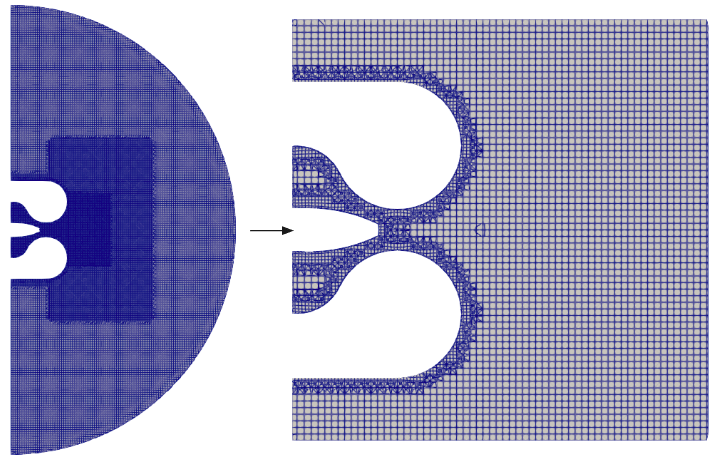
\includegraphics[width=11cm]{images/Methodology/Clipped.png}
    \caption{Depiction of the area of focus for deep learning - the original CFD mesh (left) is clipped and transformed into the region of interest (right)}
    \label{clipmesh}
\end{figure}
\begin{figure}[ht]
    \centering
    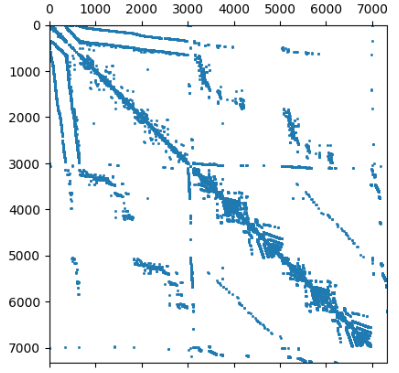
\includegraphics[width=6cm]{images/Methodology/AdjMatrix.png}
    \caption{Visualization of the adjacency matrix representing the graph connectivity of the clipped CFD mesh with 7329 nodes.}
    \label{adjmat}
\end{figure}
\subsection{Model inputs and outputs}
After data pre-processing, the simulation mesh is considered as a bidirectional graph $\mathbf{G} = (\mathbf{V}, \mathbf{E})$ where the set of $N$ nodes denoted as $\mathbf{V}$ are linked by the set of edges $\mathbf{E}$ of the mesh. To construct a graph, we need,
\begin{itemize}
\item A feature description, consolidated into an $N \times D$ feature matrix $X$ (where $N$ represents the number of nodes, and $D$ denotes the number of input features).
\item The graph connectivity or relationships within nodes is represented in matrix form as an adjacency matrix, $A$ or as an edge set $E$ of the shape $2 \times P$, where $P$ is the number of pairs of connected nodes in $E$.
\end{itemize}
Let each node have $F_X$ features, and $F_Y$ predictions. The GNN maps the set of node features and edge index matrices to predictions as, 
\begin{equation}
    \mathrm{GNN}: \mathbb{R}^{{N} \times F_{\mathrm{X}}}, \mathbb{W}^{2 \times P} \rightarrow \mathbb{R}^{{N} \times F_{\mathrm{Y}}}
    \end{equation}
We then get a graph-level output $Z$ of the shape ${N} \times F_{\mathrm{Y}}$. \\
The node feature vector $\mathbf{x}_i$ and prediction vector $\mathbf{y}_i$ of interest at each node $v_i$ is given as,
\begin{equation}
    \begin{aligned}
    & \mathbf{x}_i=\left[u_{x, i}, u_{y, i},c_{x, i}, c_{y, i}, \gamma_{\operatorname{tag}, i}\right] \\
    & \mathbf{y}_i=\left[u_{x, i}, u_{y, i}, p_i\right]
    \end{aligned}
\end{equation}
where $u_{x, i}$ and $u_{y, i}$ are the node velocities in X and Y directions, $c_{x, i}$ and $c_{y, i}$ are the spatial co-ordinates of the nodes and $p_i$ is the node pressure. $\gamma_{\operatorname{tag}, i}$ is the node tag that defines which cell the node belongs to: inlet, walls or internal mesh. To summarize, our model has 5 input channels (representing node features) and 3 output channels (denoting node predictions). In addition to these channels, the GNN model also requires an edge index matrix to internally compute the adjacency matrix for the graph. 
\subsection{Data normalization}
Data normalization is performed on both input channels (node features) and output channels (target vectors), carried out in three steps outlined below.
\begin{enumerate}
\item Following common practice, we normalize all the fields of interest with respect to the magnitude of free-stream or reference velocity $u_0$ to make them dimensionless. 
\begin{equation}
    \Tilde{u}=u /\left\|u_0\right\|, \quad \Tilde{p}=p /\left\|u_0\right\|^2
\end{equation}
The latter plays a crucial role as it eliminates the quadratic scaling effect present in the pressure values of the target data, effectively flattening the solution space, thereby simplifying the task for the neural network in subsequent stages.
\item Next, we subtract the mean pressure from the dimensionless pressure values. 
\begin{equation}
\hat{p} = \Tilde{p} - p_{mean} , \quad \text{where} \quad p_{mean} = \sum_i p_i / n
\end{equation}
$n$ is the number of training samples and $p_i$ denotes individual pressure values. Without this step, the pressure targets depict an ill-posed learning objective since the random pressure offsets in the solutions lack correlation with the inputs.
\item As a final step, every channel undergoes normalization to the range of [-1, 1] (or [0,1]). This standardization aims to mitigate errors stemming from finite numerical precision during the training period. We opt for the maximum absolute value of each quantity across the entire training dataset to normalize the data. 
\end{enumerate}
The dataset is split into 3 parts and distributed as Training data : Validation data : Test data in the ratio 80:10:10. 
\section{Graph U-Net}
Here, we introduce the Graph U-Net architecture, a foundational framework for the surrogate models used in this work. We analyze the benefits and shortcomings of this model as well as explain the motivation behind developing a modified GNN.
\begin{figure}[ht]
    \centering
    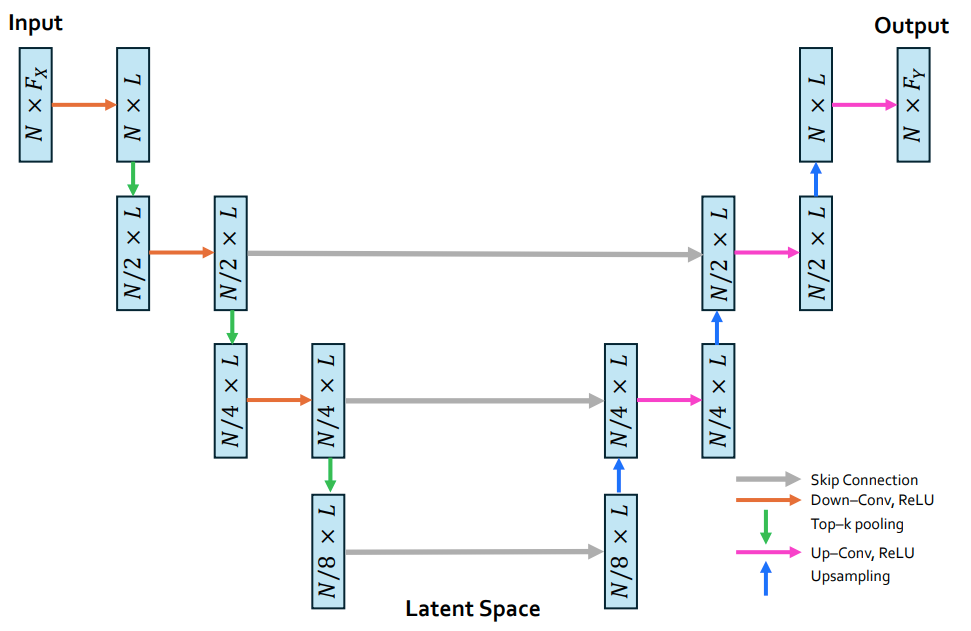
\includegraphics[width=12cm]{images/Methodology/GraphUNet.png}
    \caption{Detailed view of the Graph U-Net architecture applied to fluid dynamics, showcasing an encoder-decoder structure with skip connections. Each layer’s application is annotated with the resultant dimensions, illustrating the feature reduction or expansion throughout the network. Here, L is the number of hidden layers, N is the number of nodes in the graph, and F$_X$ and F$_Y$ denote the number of input and output features respectively.}
    \label{fig:GraphUnet}
\end{figure}
\subsection{GCNConv layer}
GCNs are NNs operating on graph-structured data that extend the concept of convolutional operations from regular grid-like data, such as images, to irregular and non-Euclidean graph structures, using the spectral graph convolution operation GCNConv. The GCNConv layer aggregates information from neighboring nodes and updates the representations of each node based on this aggregated information, expressed as,
\begin{equation}
h_i^{(l+1)} = \sigma \left(\sum_{j \in \mathcal{N}(i)} \frac{1}{c_{ij}} W^{(l)} h_j^{(l)} + B^{(l)} h_i^{(l)} \right)
\end{equation}
where $W^{(l)}$ and $B^{(l)}$ are the learnable weight and bias matrices for layer $l$, $\sigma$ is the activation function and $c_{ij}$ is a normalization factor. 
In contrast to filters in CNNs, the weight matrix is consistent and shared across all nodes. However, unlike pixels, nodes do not have a fixed number of neighbors. To maintain uniform value ranges across all nodes and facilitate comparability between them, we normalize the outcomes based on the degree of the nodes, i.e; the number of connections of each node. Hence, $c_{ij} = \sqrt{deg(i)}\sqrt{deg(j)}$ where, ${deg(i)}$ and ${deg(j)}$ denotes the degree of the nodes $v_i$ and $v_j$ respectively. 
% Some important aspects of graph convolutions are detailed below. 
% \begin{enumerate}
% \item \textbf{Aggregation of neighbor information:} Each node aggregates the features of its neighbors, weighted by the parameters learned in the weight matrix $W^{(l)}$. This process enables nodes to incorporate information from their local neighborhoods, capturing relational dependencies and structural patterns in the graph. 

% % The normalization factor $c_{ij}$ ensures that the aggregated features are appropriately scaled based on the connectivity of nodes.
% \item \textbf{Weight sharing:}
% The weight matrix $W^{(l)}$ is shared across all nodes, allowing the model to capture common patterns and relationships present in the graph. By sharing parameters, GCNs can effectively learn representations from limited labeled data, facilitating transfer learning and adaptation to new graphs or domains.
% \item \textbf{Hierarchical feature learning:}
% GCNConv layer enables hierarchical feature learning by iteratively aggregating information from neighboring nodes. As information propagates through multiple layers, nodes can capture increasingly abstract and high-level features of the graph. 
% \end{enumerate}
\subsection{Downsampling}
The downsampling operation is carried out using the top-k pooling strategy, which retains the most important nodes in the graph while discarding less relevant nodes based on a specified criterion. It uses a pooling ratio approach such that the graph has $\lfloor kN \rfloor$ nodes after the pooling operation, where $k \in (0, 1]$ is the pooling ratio. The decision of which nodes to discard is based on a projection score computed against a learnable vector, $\mathbf{\overrightarrow{p}}$. Fully expressed, computing a pooled graph, $(X^l, A^l)$, from an input graph, $(X, A)$ can be described using the following algorithm: 
\begin{enumerate}
    \item Compute a score for each node in the graph based on node importance or feature relevance as,
    \[
\mathbf{\tilde{y}} = \frac{X \mathbf{\overrightarrow{p}}}{k||\mathbf{\overrightarrow{p}}||_2} \]
    \item Select the top $k$ nodes with the highest scores, \[ \mathbf{\overrightarrow{i}} = \text{top-k}(\mathbf{\tilde{y}}, k) \]
    Discard the remaining nodes and their associated edges, resulting in a downsampled graph $G^{\prime} = (V^{\prime}, E^{\prime})$ where $V^{\prime}$ contains only the selected nodes.
    \item Retain the features corresponding to the selected nodes to form the downsampled feature and adjacency matrices, \[
        X^{\prime} = (X \odot \tanh(\mathbf{\tilde{y}}))_{\mathbf{\overrightarrow{i}}}, \quad A^{\prime} = A_{\mathbf{\overrightarrow{i}},\mathbf{\overrightarrow{i}}}
       \]
\end{enumerate}
Here, $||.||_2$ represents the L$_2$ norm, $\odot$ denotes element-wise multiplication, and $\cdot_{\mathbf{\overrightarrow{i}}}$ represents an indexing operation that extracts slices at indices specified by $\mathbf{\overrightarrow{i}}$. 
\subsection{Upsampling}
In the Graph U-Net architecture, unpooling is not a distinct operation like in traditional U-Nets. Instead, skip connections are used to implicitly perform unpooling. During decoding, downsampled features from the encoder are combined with zeros or empty features in the decoder using skip connections. This integration effectively restores spatial details and contextual information from the original input graph, ensuring that important features are retained and allowing for the recovery of detailed graph structures. Therefore, unpooling in Graph U-Net is seamlessly integrated into the skip connection mechanism, facilitating the reconstruction of the original graph resolution during decoding.
\subsection{Results and discussion}
For the surrogate model that exactly uses the Graph U-Net architecture, we are initially interested in investigating the ability of the model to reproduce the target data, i.e; when the same target data is given as input. This means that the task solely performs reconstruction of the target dataset, without requiring to predict something. We also go on to perform the prediction task with this model, which forms the baseline for all the other architectures proposed in this work. The following settings are maintained for both the reconstruction and prediction tasks. We implement a 9-fold cross-validation for the training process. The initial learning rate is set to $0.0005$ and a Step LR scheduler is used to decay the learning rate by a factor of $0.75$ after every 100 epochs. We use the Adam optimizer and train on the \gls{RMSE} loss for 500 epochs. The model's hyperparameters are selected by a hyperparameter tuning process. Table \ref{table:complex} presents the model complexity and performance on varying the number of channels and hidden layers. It is to be noted that, each hidden layer refers to the combination of sampling (pooling and unpooling) and convolution operations (up and down convolutions). That is, if we perform the pooling and convolutions $d$ times in the encoder and reverse this process $d$ times in the decoder, the number of hidden layers in this architecture is taken as $d$.
\begin{table}[ht]
    \centering
    \caption{Hyperparameter tuning - Table depicting the number of channels, hidden layers, trainable parameters and the training loss measured with the RMSE criterion for the Baseline architecture corresponding to each setting.}
    \label{table:complex}
    \begin{tabular}{|c|c|c|c|}
    \hline
    \textbf{Channels} & \textbf{Hidden layers} & \textbf{Trainable parameters} & \textbf{Training loss} \\
    \hline
    \multirow{4}{*}{48} & 2 & 7k &  0.04876\\
    \cline{2-4}
                        & 3 & 12k &  0.04713\\
    \cline{2-4}
                        & 4 & 17k & 0.04386\\
    \cline{2-4}
                        & 5 & 22k &  0.04272 \\
    \hline
    \multirow{4}{*}{64} & 2 & 13k & 0.04536\\
    \cline{2-4}
                        & 3 & 21k & 0.05074 \\
    \cline{2-4}
                        & 4 & 30k &  0.04139\\
    \cline{2-4}
                        & 5 & 31k & 0.04692 \\
    \hline
    \multirow{4}{*}{128} & 2 & 51k& 0.03983\\
    \cline{2-4}         
                         & 3 & 84k & 0.03840\\
    \cline{2-4}
                         & 4 & 117k & 0.03642  \\
    \cline{2-4}
                         & 5 & 150k &  0.05011\\
    \hline
    \end{tabular}
    
    \end{table}

Among the models with similar performance, we choose the one that is the simplest, i.e; has relatively lesser trainable parameters, without compromising on the accuracy or facing the risk of overfitting. Hence, we execute the training process using a GNN architecture with 128 channels and carry out the sampling and convolution operations 3 times (number of hidden layers) on the encoder and the decoder side. Similar experiments have been conducted to choose the ideal batch size, activation function and other hyperparameters. The key hyperparameters are listed in Table \ref{table:hp}. 
\begin{table}[ht]
    \centering
    \caption{Model hyperparameters}
    \label{table:hp}
    \begin{tabular}{|l|l|}
    \hline
    \textbf{Hyperparameter}    & \textbf{Value/Description} \\
    \hline
    Channels    & 128                           \\
    \hline
    Hidden layers    & 3                          \\
    \hline
    Pooling ratios             & [0.5,0.5,0.5,0.5,0.5]                       \\
    \hline
    Batch size                 & 4                         \\
    \hline
    Activation function        & ReLU                       \\
    \hline
    Weight initialization    &  Kaiming                        \\
    \hline
    Initial learning rate       & 0.0005                       \\
    \hline
    \end{tabular}
    \end{table}
The training, validation loss are quantified with the \gls{RMSE} heuristic as the average over 9 folds after 500 epochs. 
\subsubsection{Reconstruction task}
As mentioned previously, we prescribe the same dataset (simulation results at 30000 time-steps) as the input and target data to evaluate the effectiveness of reconstruction of the Graph U-Net model. The CFD results, predictions of the GNN model and the absolute difference between these data for a simulation case from the test dataset with 18 m/s and 27 m/s as the inlet 1 and inlet 2 velocities respectively are shown in Figure \ref{blrecon}.
\begin{figure}[ht]
    \centering
    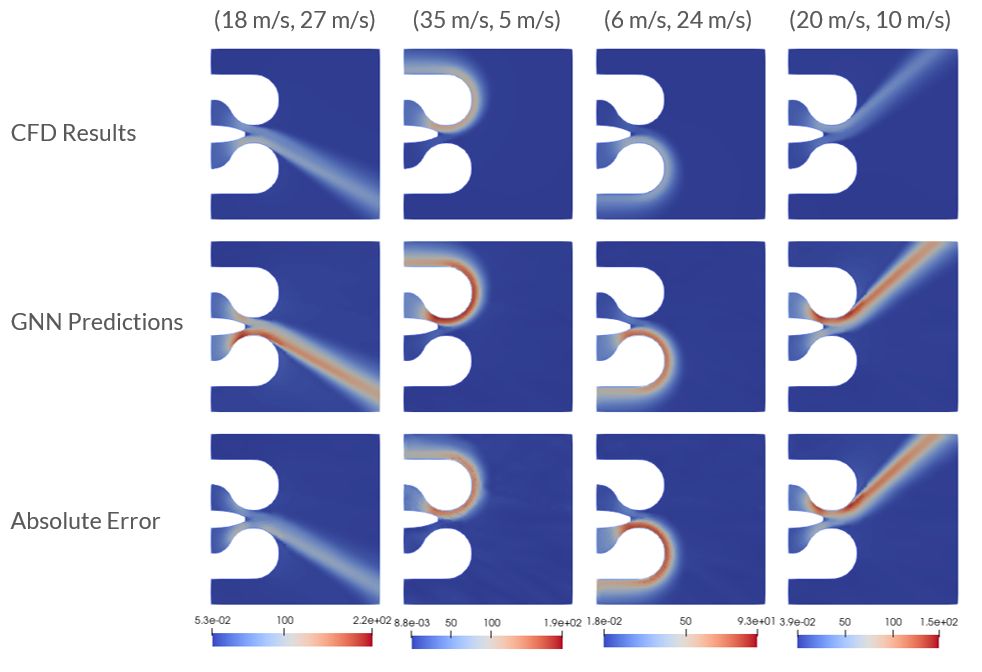
\includegraphics[width=14cm]{images/Methodology/allvelrecon.png}
    \caption{Visualization of velocity fields for four cases from the baseline's reconstruction task, with inlet velocity values prescribed as (Inlet 1, Inlet 2) presented in four columns. Here, the first row represents results the target data, the second row corresponds to the GNN predictions for the velocity field, and the last row is the absolute difference between the target data and GNN predictions. The colours signify the magnitude of velocity, mapped by the legend.} 
    \label{blrecon}
\end{figure}
We observe that although the GNN reconstructs the trends of the outflow jet similar to the target data, the scale or the range of velocity magnitude are slightly different for the two cases. Thus, the baseline model is unable to accurately capture the velocity fields for reconstruction. The poor reconstruction can be attributed to the lack of explicit unpooling layers in Graph U-Net, which can lead to inadequate reconstruction of the original graph structure during decoding. 
\subsubsection{Prediction task}
In this case, we predict the steady-state solutions from the earlier time step. The CFD results, predictions of the GNN model and the absolute difference between these data for four simulation cases from the test dataset are shown in Figure \ref{blpred}.
\begin{figure}[ht]
    \centering
    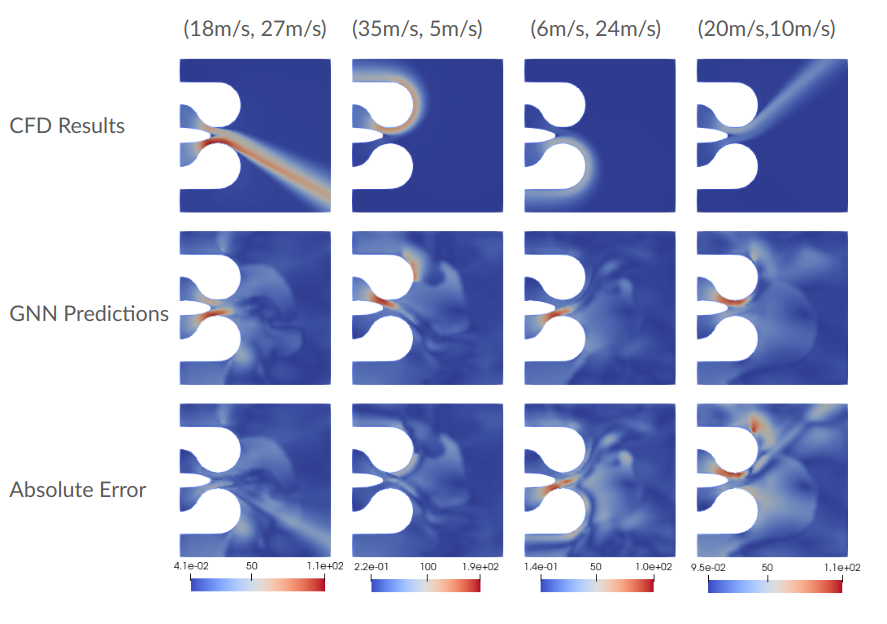
\includegraphics[width=14cm]{images/Methodology/Baselineprediction.png}
    \caption{Visualization of velocity fields for four cases from the baseline's prediction task, with inlet velocity values prescribed as (Inlet 1, Inlet 2) presented in four columns. Here, the first row represents results the target data, the second row corresponds to the GNN predictions for the velocity field, and the last row is the absolute difference between the target data and GNN predictions. The colours signify the magnitude of velocity, mapped by the legend.} 
    \label{blpred}
\end{figure}
As we can understand from the figure, the predicted direction of the outflow jet as well as its magnitude vary significantly from the expected target data. Thus, the baseline model is not feasible for the prediction task of nozzle flow dynamics. To better comprehend and evaluate the model performance, we estimate the training, validation and test losses of the baseline model for both the tasks in Table \ref{table:perform}. Furthermore, we note down the absolute difference between the input and target data for the test dataset of the prediction task. Some other limitations to this architecture are,  

\begin{table}[ht]
    \centering
    \caption{Model evaluation metrics of the Baseline model for the reconstruction and prediction tasks.} 
    \label{table:perform}
    \begin{tabular}{|l|l|l|l|l|}
    \hline
    \textbf{Model} & \textbf{Training Loss} & \textbf{Validation Loss} & \textbf{Test Loss} & \textbf{Abs Difference} \\
    \hline
    Baseline - Reconstruction & 0.025627 & 0.028391 & 0.029312 & 0\\
    \hline
    Baseline - Prediction & 0.1459 & 0.1503 & 0.1635 & 0.2626\\
    \hline
    \end{tabular}
    \end{table}
    
\begin{enumerate}
    \item \textbf{Limited scalability:} Originally designed for small graphs with around 100 nodes, Graph U-Net relies on dense matrix multiplications, which are memory-intensive and not scalable. This leads to memory constraints and slower training times, thus making it impractical for complex, large-scale graph data.
    \item \textbf{Computational overhead:} Graph U-Net conducts dense adjacency matrix multiplication in the forward pass, resulting in longer training and inference times.
    \item \textbf{Limited expressiveness:} GCNConv layers may have limited expressiveness in capturing higher-order graph structures and capturing long-range dependencies in the graph. Its optimal depth is found to be 2 or 3 layers \cite{kipf}. Deeper models beyond 7 layers can encounter training difficulties due to heightened risk of overfitting.
\end{enumerate}
Due to these disadvantages, Graph U-Net may exhibit poor performance in terms of both accuracy and efficiency, particularly for complex geometries or large datasets. Hence, there is a paramount necessity to rely on modified GNN architectures for our work.
\section{Proposed architecture}
\label{proparch}
In this section, we propose three GNN surrogate models and elucidate the components in the architecture and the modifications made on the original Graph U-Net framework. Then, we proceed to provide details on the hyperparameters and other implementation specifics of the proposed GNN models. Finally, we demonstrate the training process and share the predictions, training and test results obtained for the CFD application. The models are developed on the Pytorch deep learning framework using the Pytorch Geometric (PyG) library. Training and testing are performed on a compute node of the \gls{HPC} cluster Loewenburg, using a single nVidia Tesla V100 GPU. \\
There are 3 different surrogate models proposed and each of them tackle the unpooling limitation in Graph U-Net by using a \gls{k-NN} approach for upsampling used in PointNet++ \cite{pnpp}, with k set to 3. The downsampled features at different depths (levels of coarsening) are stored so that the upsampled node co-ordinates required for k-NN interpolation can be obtained from $[c_{x}, c_{y}]$ at the downsampled feature of the same depth. The architectures also include skip connections, although they do not perform the task of upsampling here. The three surrogate models differ in the convolutional operations used, as described below. 
\begin{enumerate}
    \item \textit{Graphknn} uses GCNConv layers as used in Graph U-Nets to perform convolutions and executes the upsampling operation with the help of k-NN interpolation. 
    \item The \textit{SAGEknn} surrogate model replaces the GCNConv layers of Graph U-Net with GraphSAGE convolutional layers from \cite{SAGE} and also implement the k-NN interpolation for unpooling. 
    \item In \textit{MoNetknn}, we carry out convolution operations using the GMMConv convolutional layers from \gls{MoNet} \cite{MoNet}. Additionally, we also add the k-NN interpolation function in our architecture for upsampling the features and edge indices. 

    % \item \textit{BL + crsn + knn:} In this surrogate, we first obtain the set of coarsened meshes through incremental decimation of the CFD mesh by running a Python script on Paraview. With the mesh indices and co-ordinates of the low-resolution mesh nodes, we compute the downsampled features for the graph using the sampling operator described in the subsection \ref{SO}. Thus, we implement the pooling operation with the help of sampling operator and perform unpooling operation using k-NN interpolation. 
    % \item \textit{BL + SAGE + crsn + knn:} Similar to the previous model in every detail, the only difference in this model is that it uses GraphSAGE layers instead of the GCNConv layers as convolutions.
    % \item \textit{BL + MoNet + sampl. + knn:} This model is also similar to \textit{BL + crsn + knn}, but it applies MoNet blocks for up convolutions and down convolutions. 
\end{enumerate}
We perform hyperparameter tuning for each of the architectures to arrive at the ideal choice of design parameters. The salient features of the three architectures along with their hyperparameters are tabulated in Table \ref{prophp}. 
% \subsection{Multi-Resolution Graph Net Architecture}
% \section{Model hyperparameters and training parameters}
\begin{table}[ht]
    \centering
    \caption{Features and hyperparameters comparison of 1. \textit{Graphknn}, 2. \textit{SAGEknn}, and 3. \textit{MoNetknn} architectures.}
    \label{prophp}
    \begin{tabular}{|l|l|l|l|}
    \hline
    \textbf{Feature/Hyperparameter}    & \textit{Graphknn} & \textit{SAGEknn}   & \textit{MoNetknn} \\
    \hline
    Channels    & 48 & 48 & 128                           \\
    \hline
    Hidden layers    & 3 & 3 & 4                          \\
    \hline
    Convolution layer             &     GCNConv & SAGEConv & GMMConv                   \\
    \hline
    Pooling operation             &    Top-k &  Top-k &  Top-k                     \\
    \hline
    Unpooling operation         &   k-NN interpolation&   k-NN interpolation&   k-NN interpolation                     \\
    \hline
    Batch size                 & 4 & 4& 4                         \\
    \hline
    Activation function        & ReLU  & ReLU  & ReLU                       \\
    \hline
    Weight initialization    &  Kaiming &  Kaiming &  Kaiming                        \\
    \hline
    Initial learning rate       & 0.0005 & 0.0005 & 0.001                        \\
    \hline
    \end{tabular}
    \end{table}
\section{Results and discussion}
Similar to the baseline surrogates, we perform a 9-fold cross-validation on the training and validation datasets. The optimizer, scheduler, and the loss metric remain the same as the baseline experiments. Figures \ref{allvel1}, \ref{allvel2}, \ref{allvel3} and \ref{allvel4} depict the prediction results and the absolute errors obtained from the three surrogates for four different flow conditions. 
% \subsection{Parameter study of graph layers}
% The design choices in the model architecture can impact the overall performance of the model. 
\begin{figure}[ht]
    \centering
    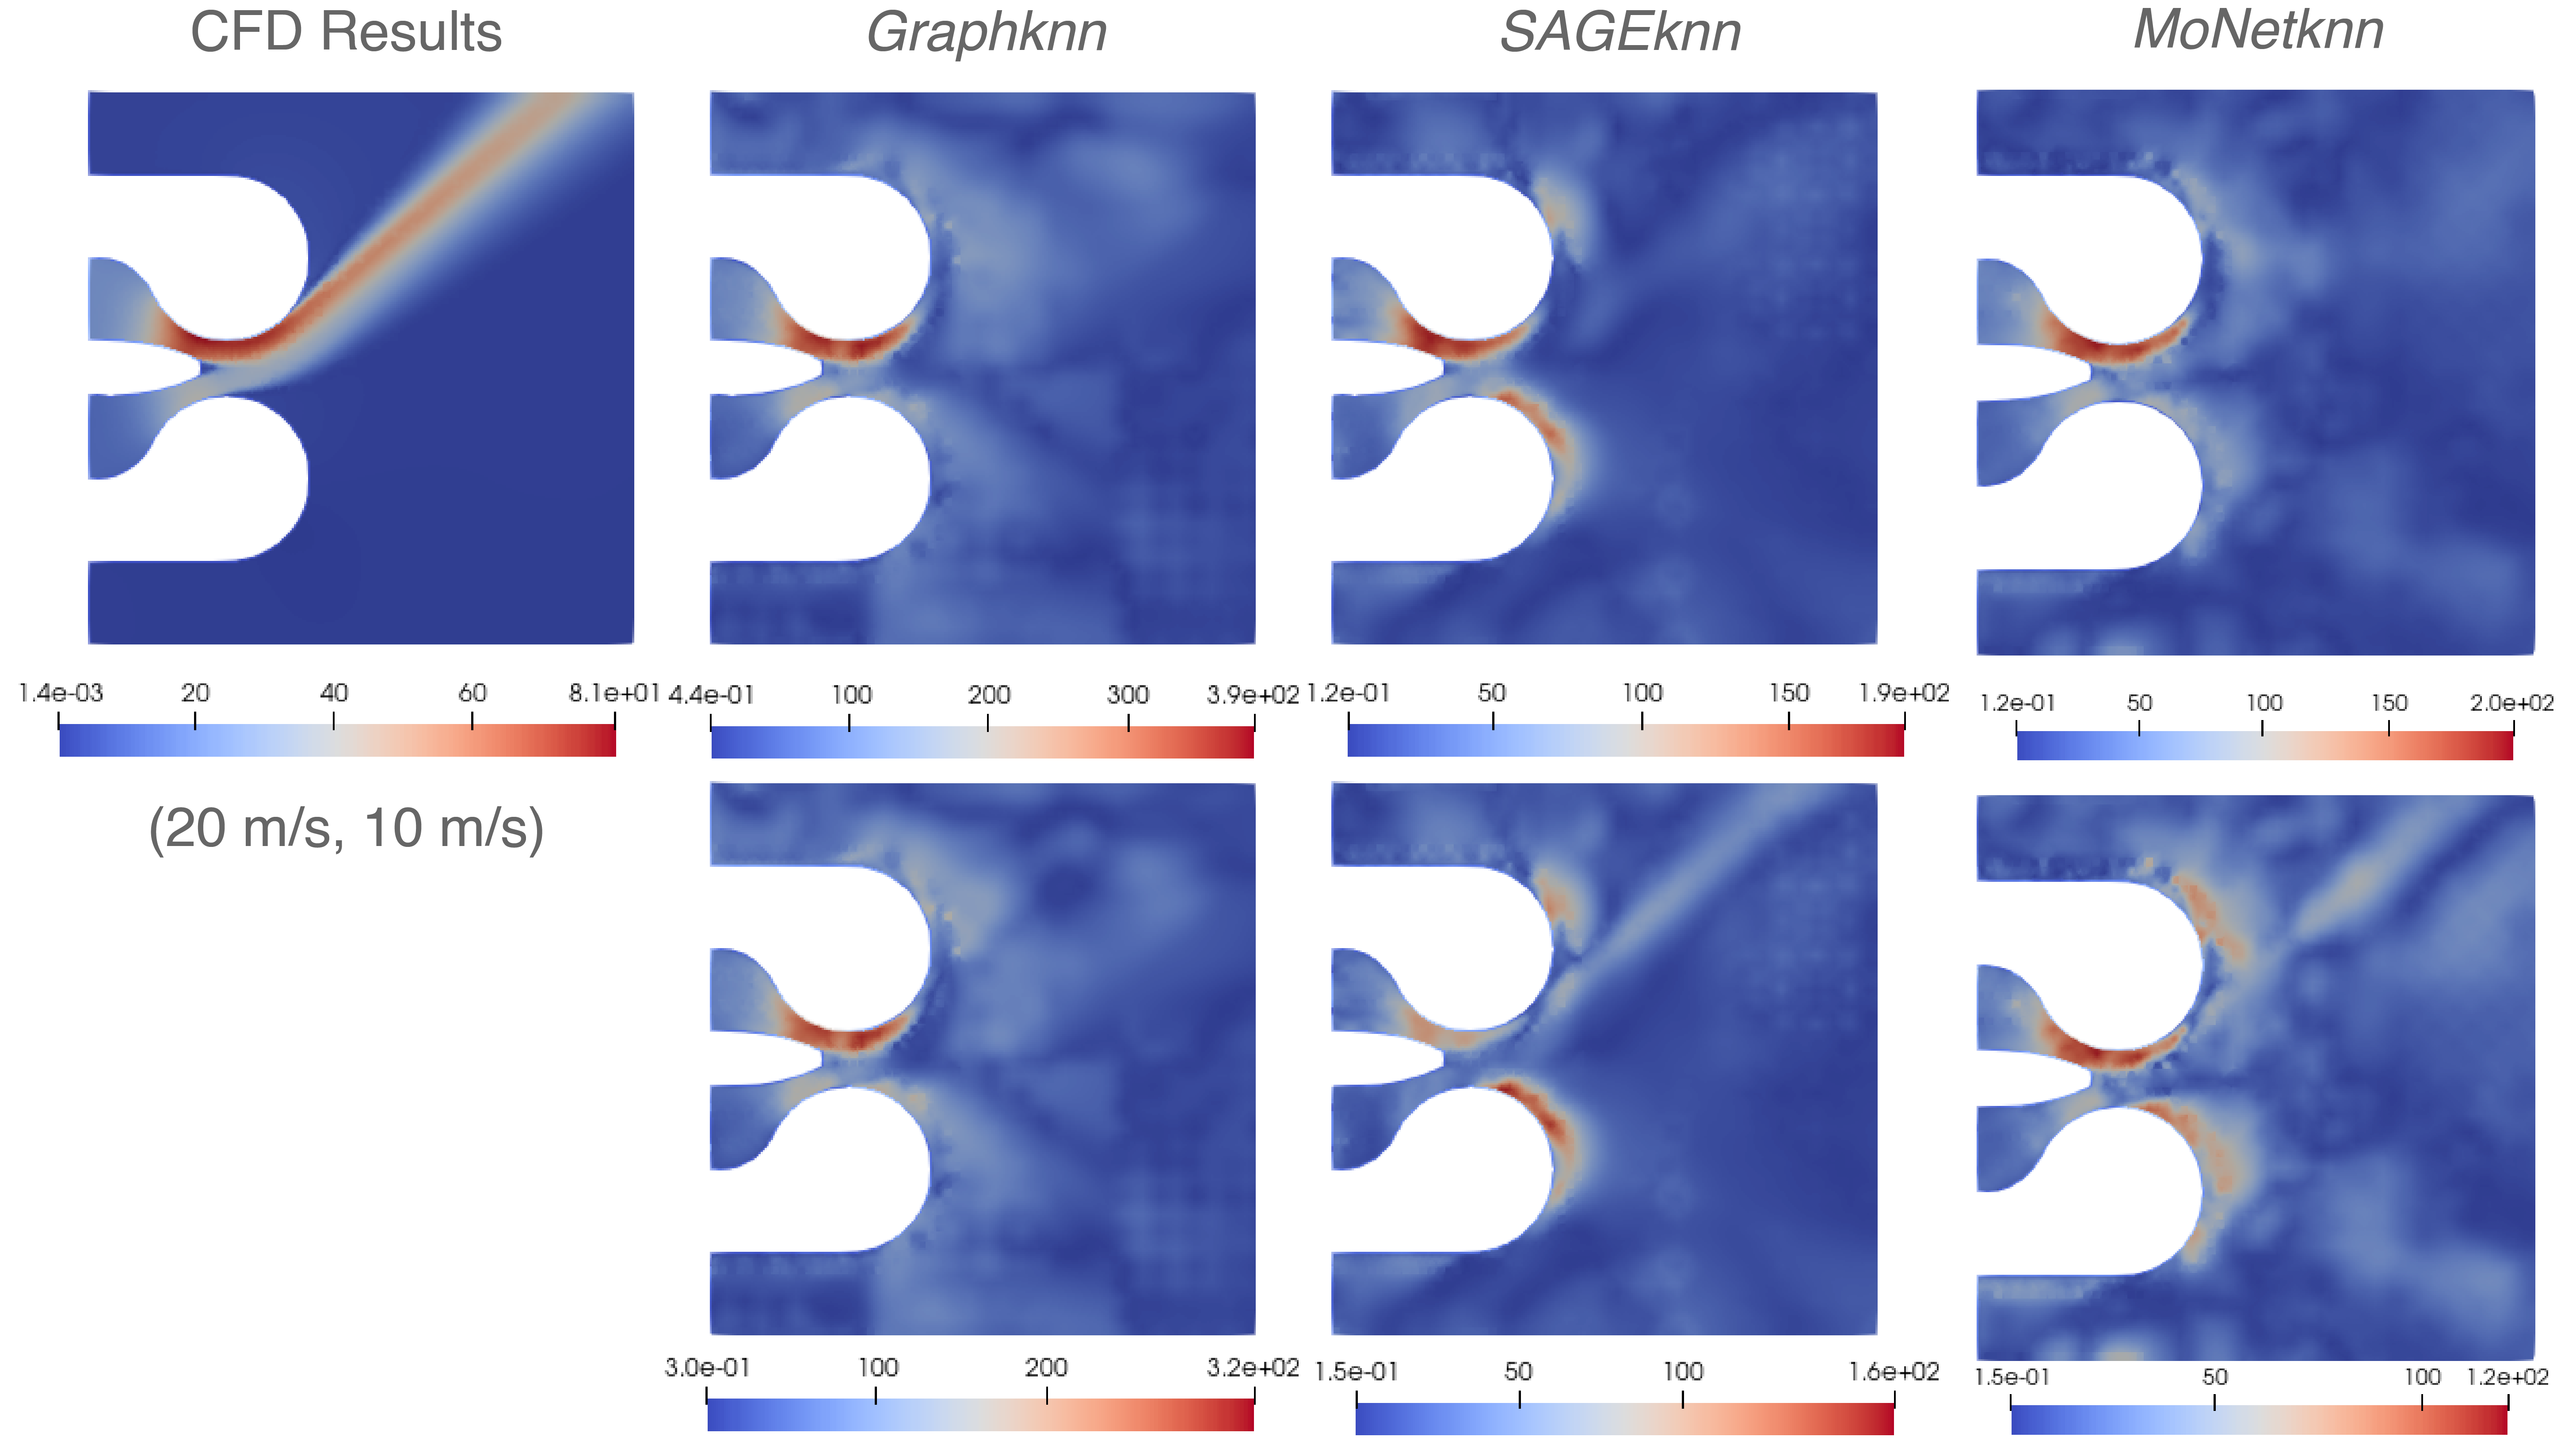
\includegraphics[width=14cm]{images/Methodology/Asset 18.png}
    \caption{Visualization of velocity fields for simulation case with (Inlet 1, Inlet 2) = (20 m/s, 10 m/s) Here, the first row represents results the target data, the second row corresponds to the GNN predictions for the velocity field, and the last row is the absolute difference between the target data and GNN predictions.} 
    \label{allvel1}
\end{figure}
\begin{figure}[ht]
    \centering
    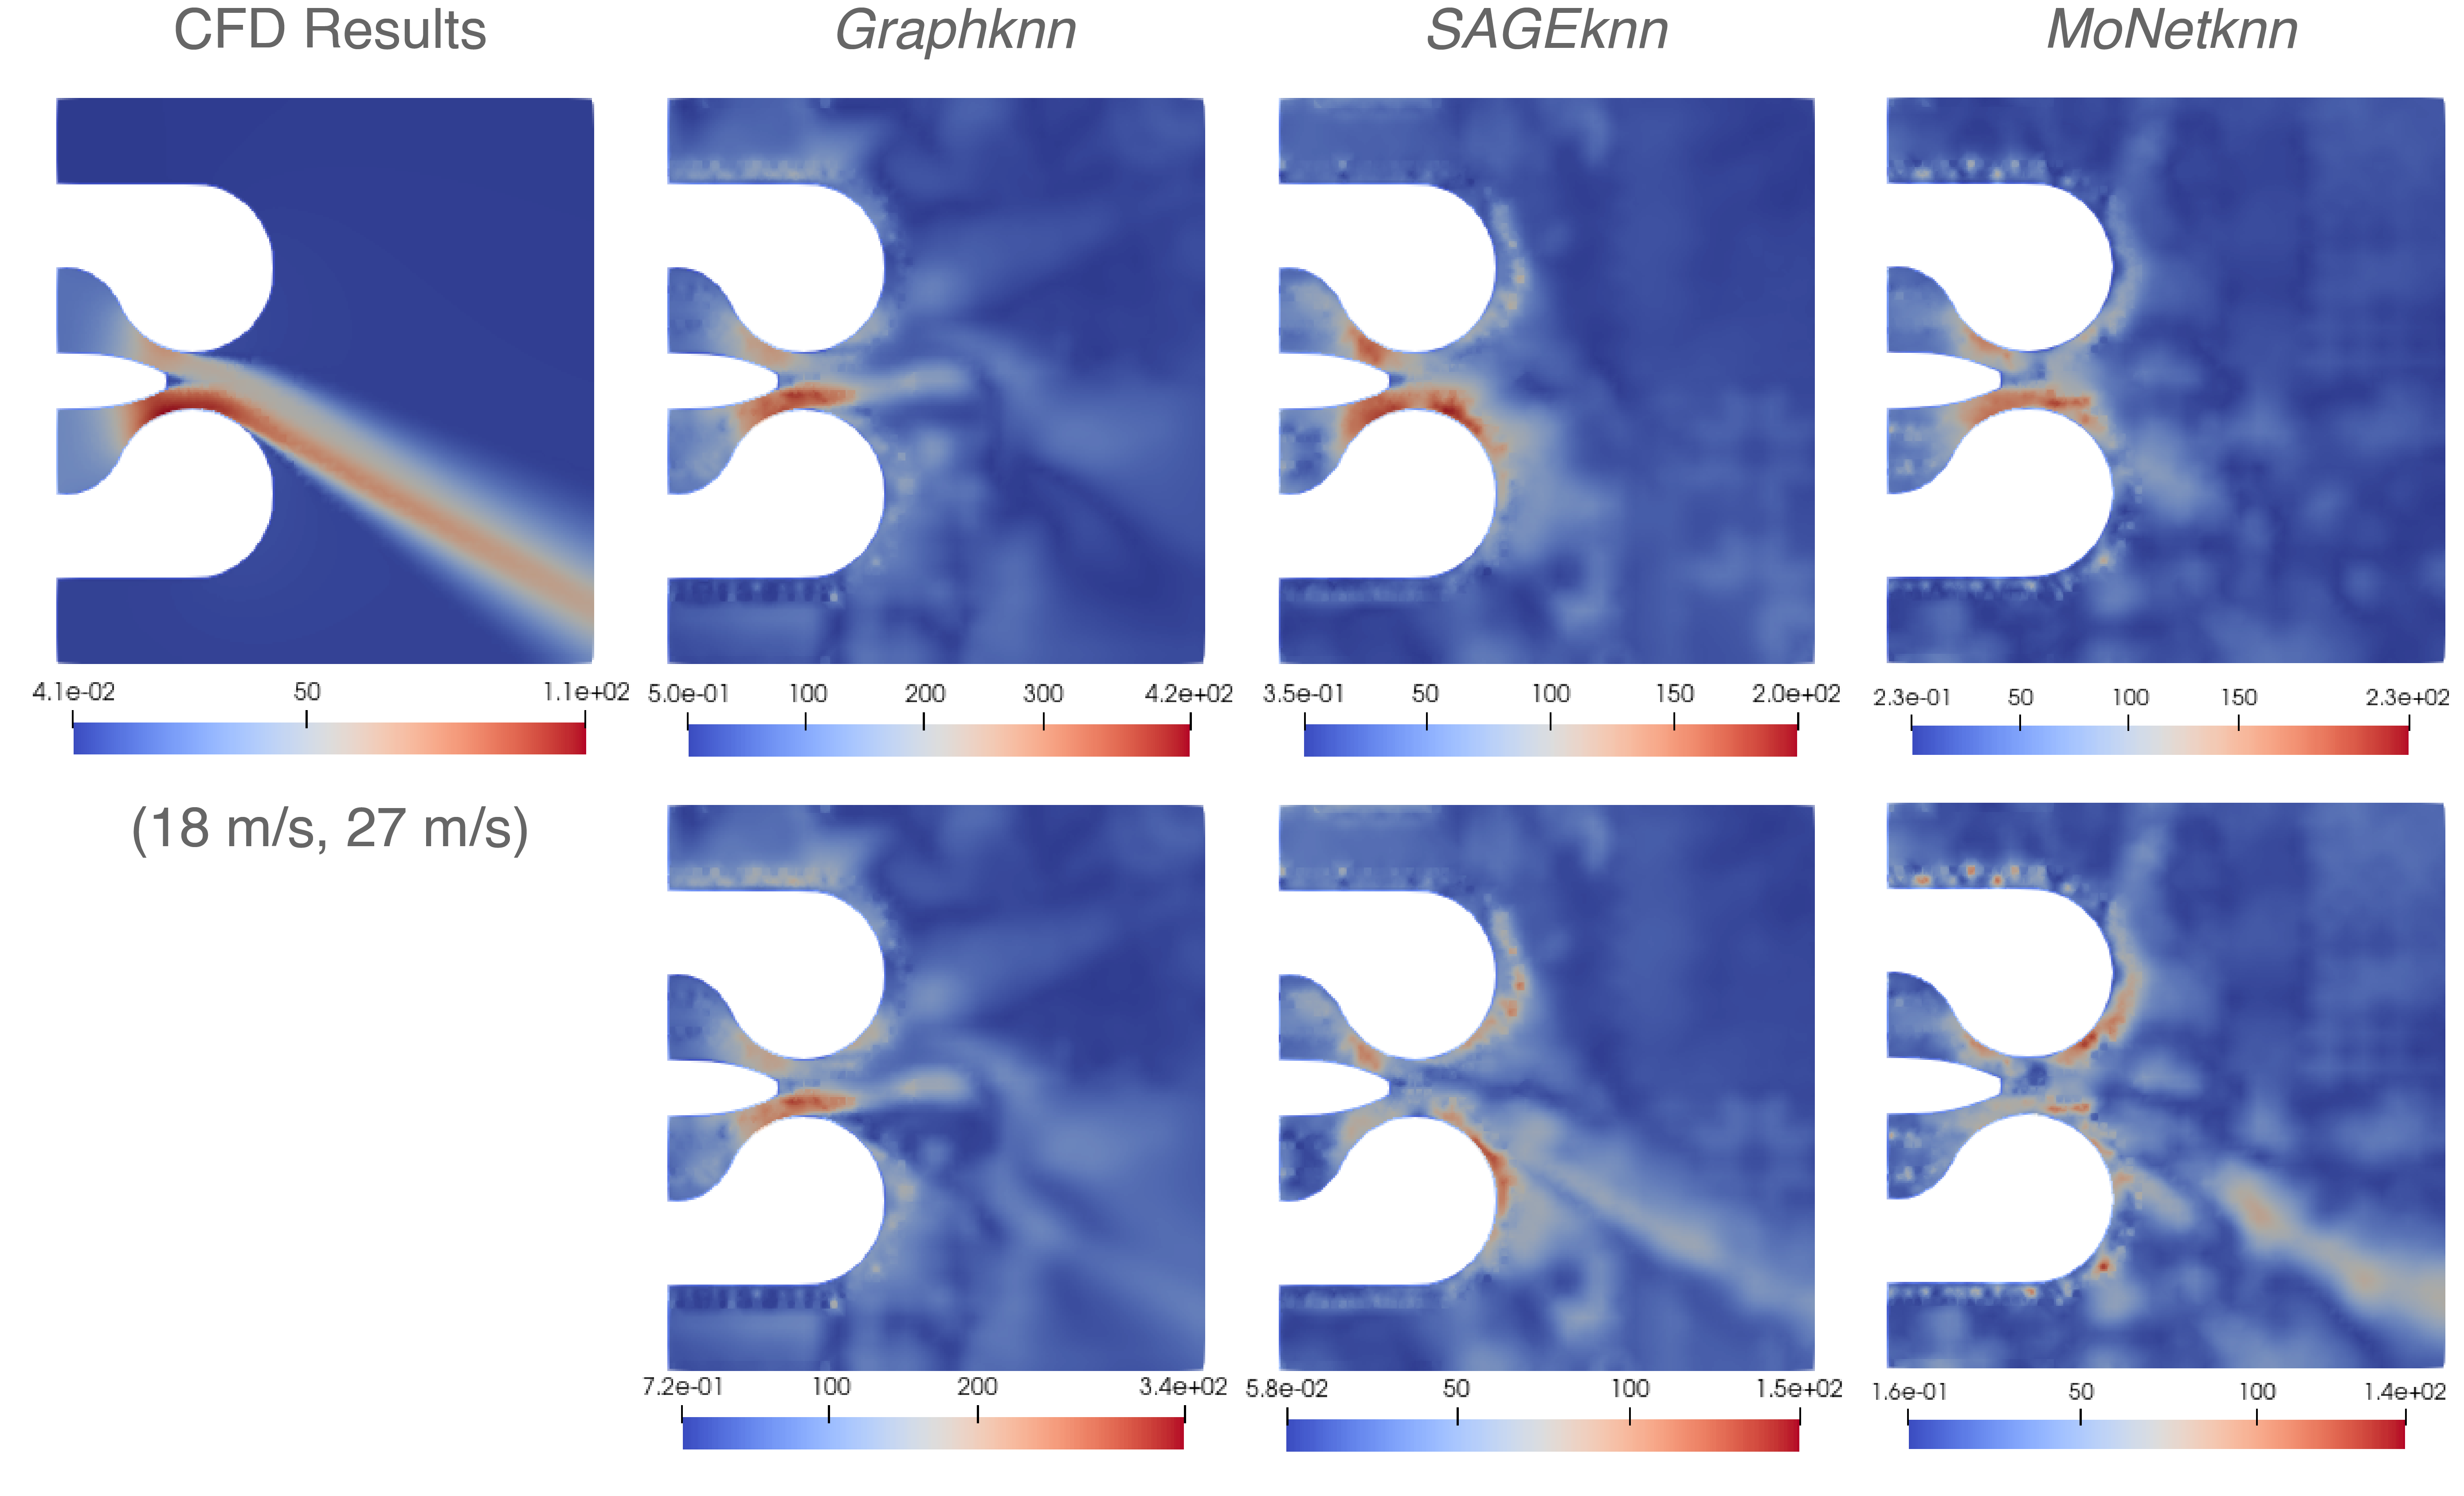
\includegraphics[width=14cm]{images/Methodology/Asset 17.png}
    \caption{Visualization of velocity fields for simulation case with (Inlet 1, Inlet 2) = (18 m/s, 27 m/s). Here, the first row represents results the target data, the second row corresponds to the GNN predictions for the velocity field, and the last row is the absolute difference between the target data and GNN predictions}. 
    \label{allvel2}
\end{figure}
\begin{figure}[ht]
    \centering
    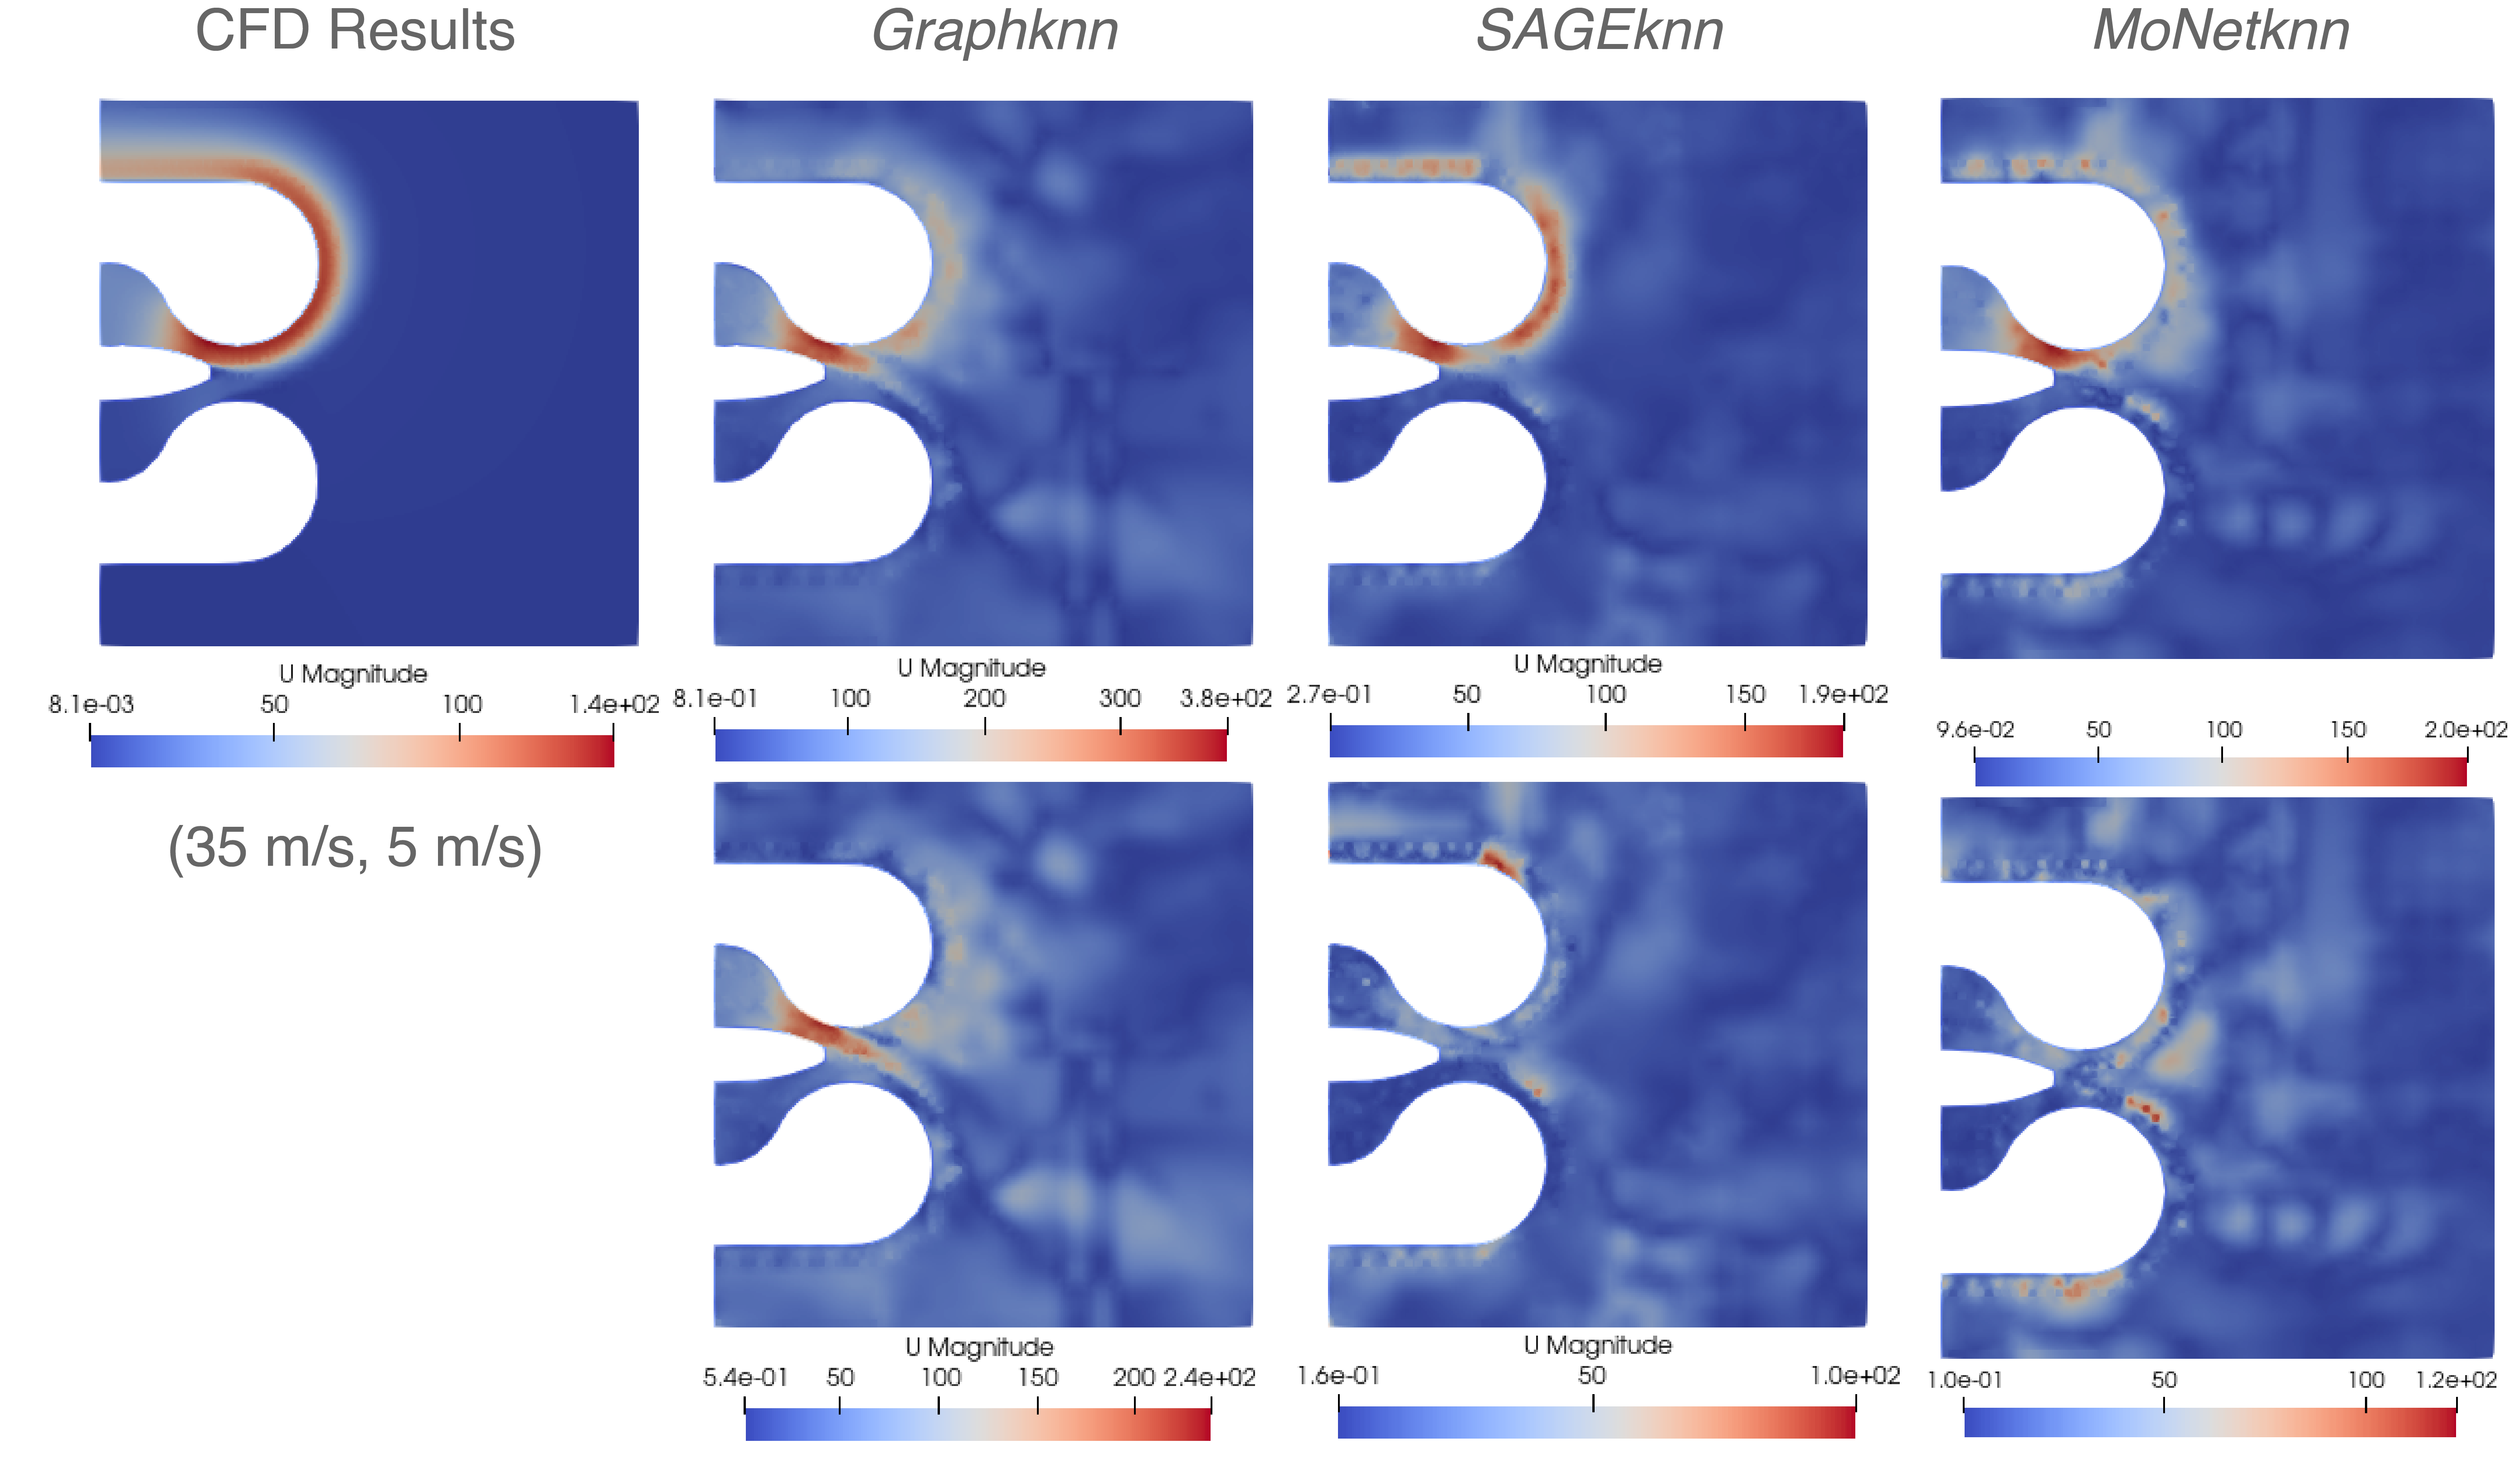
\includegraphics[width=14cm]{images/Methodology/Asset 15.png}
    \caption{Visualization of velocity fields for simulation case with (Inlet 1, Inlet 2) = (35 m/s, 5 m/s). Here, the first row represents results the target data, the second row corresponds to the GNN predictions for the velocity field, and the last row is the absolute difference between the target data and GNN predictions.} 
    \label{allvel3}
\end{figure}
\begin{figure}[ht]
    \centering
    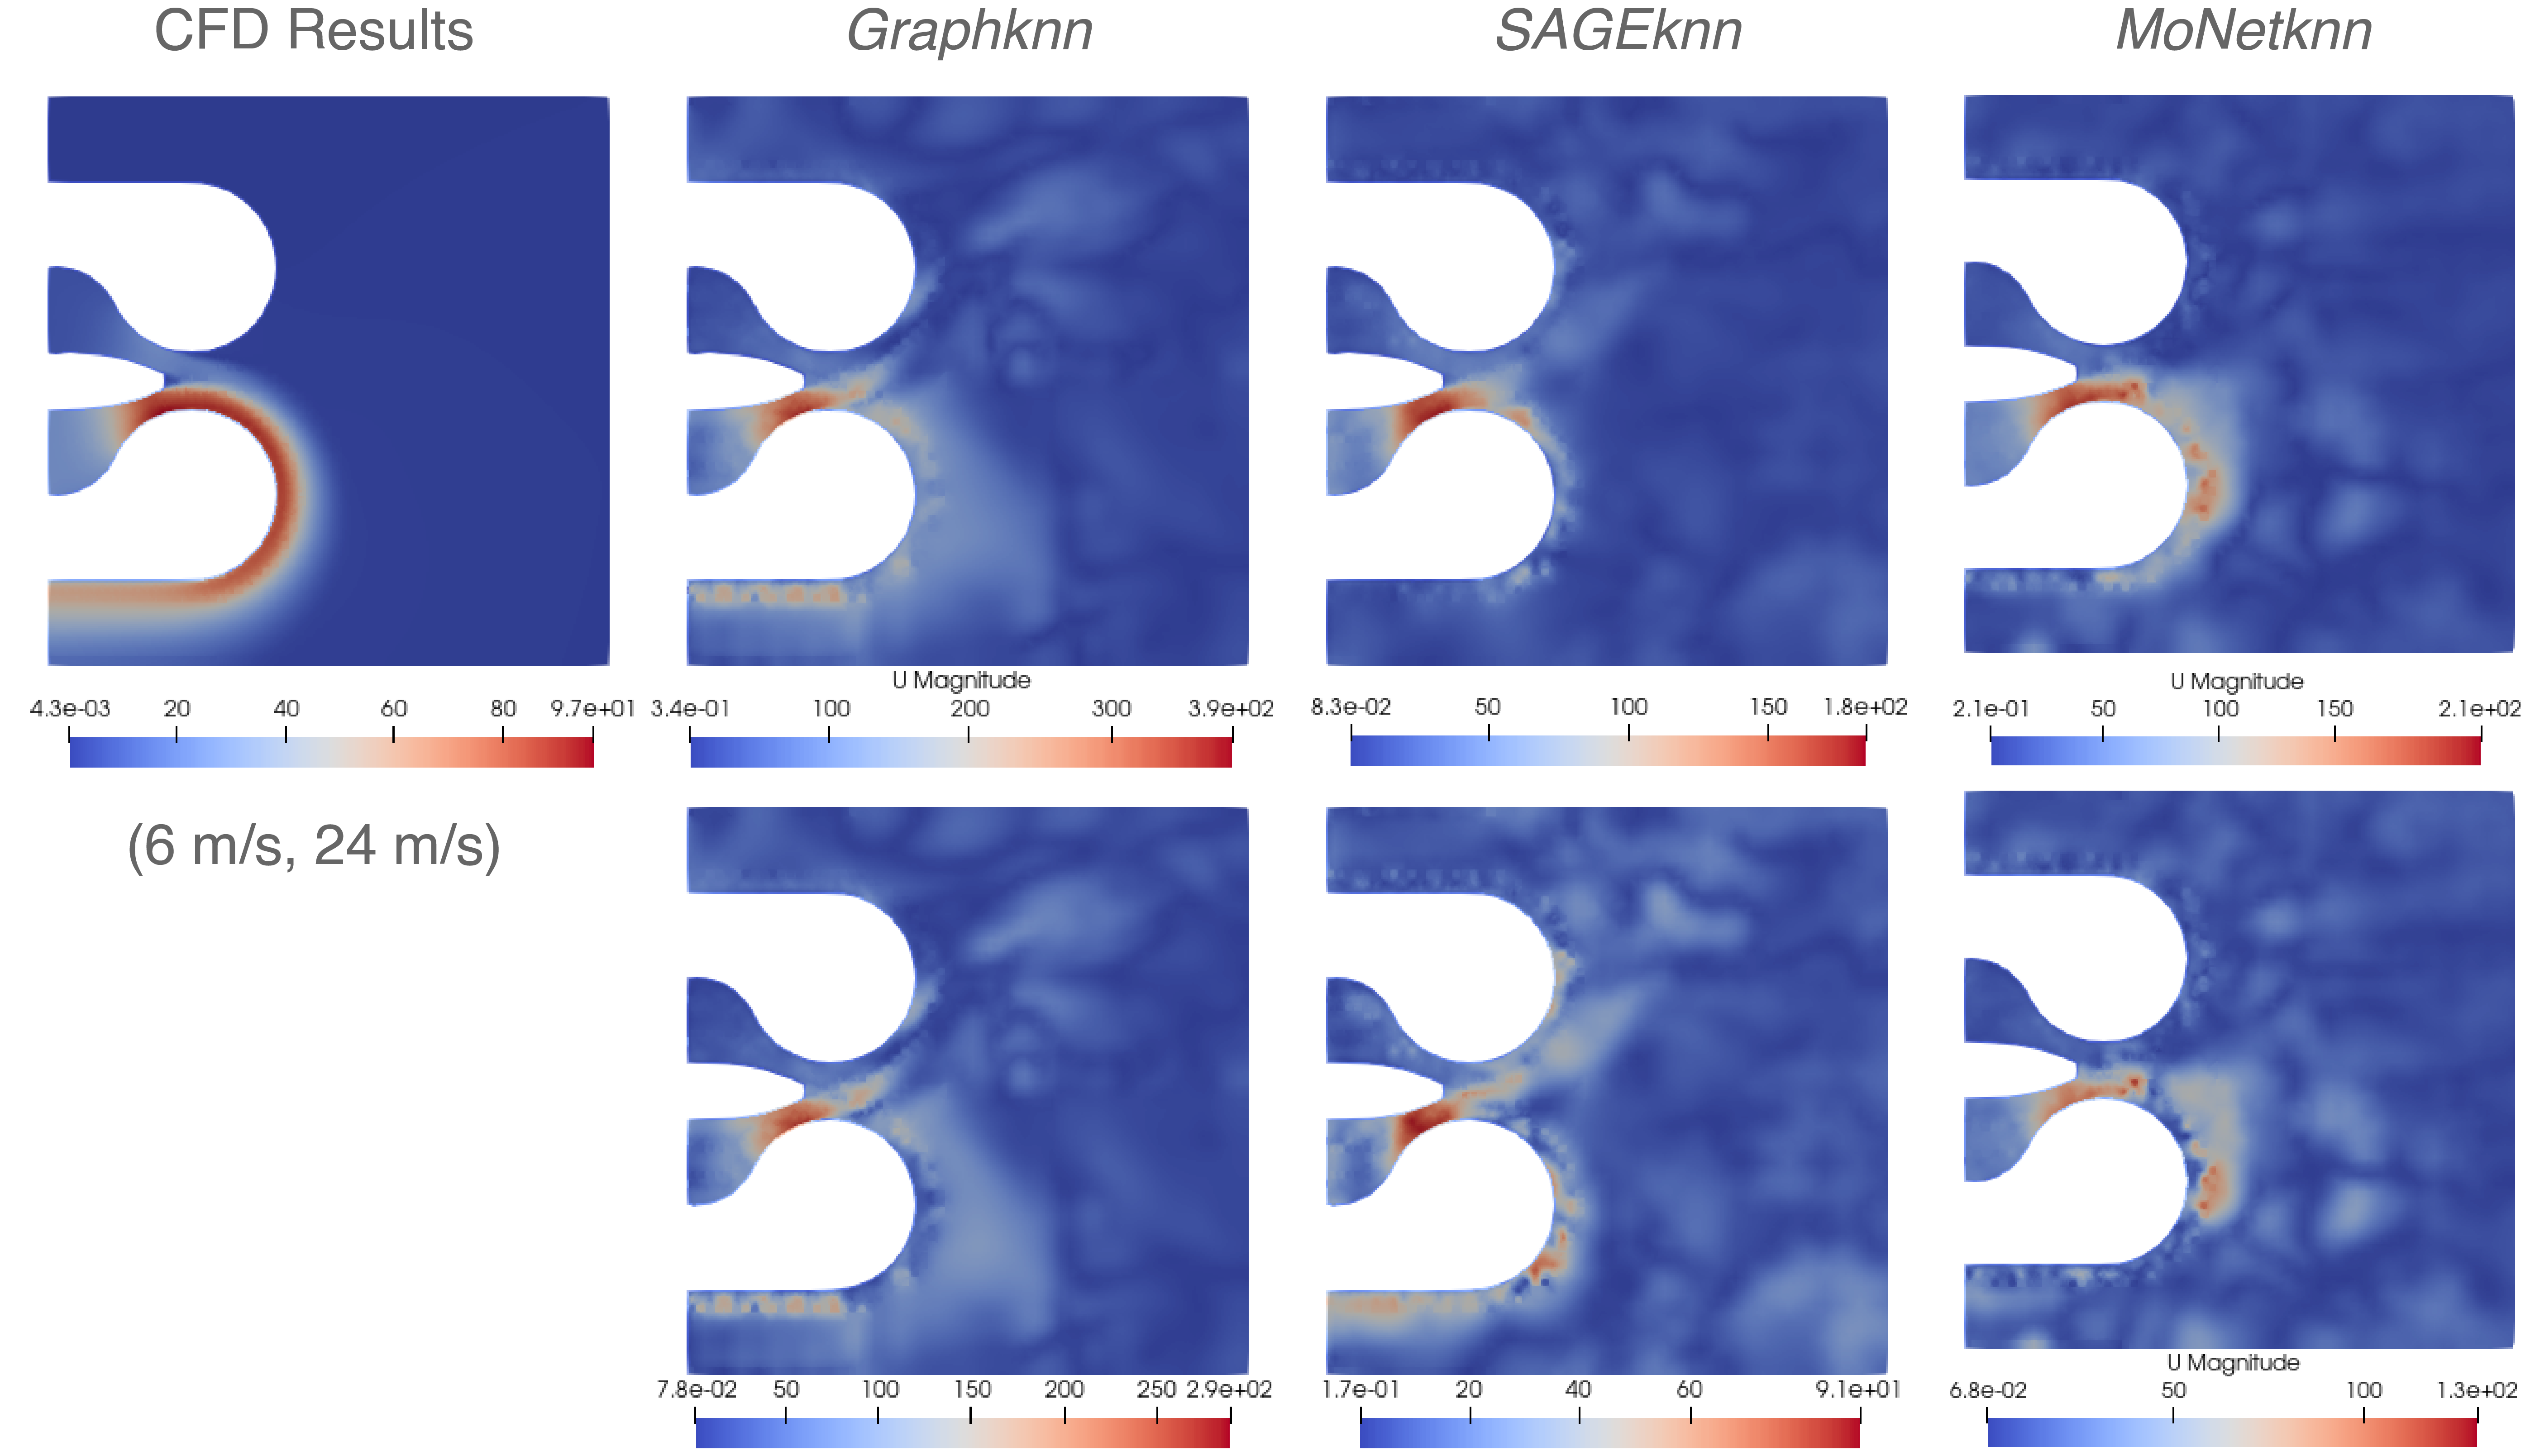
\includegraphics[width=14cm]{images/Methodology/Asset 14.png}
    \caption{Visualization of velocity fields for simulation case with (Inlet 1, Inlet 2) = (6 m/s, 24 m/s) Here, the first row represents results the target data, the second row corresponds to the GNN predictions for the velocity field, and the last row is the absolute difference between the target data and GNN predictions.} 
    \label{allvel4}
\end{figure}
To discern the performance of these models, we compute the \gls{RMSE} loss over the training, validation and test datasets, denoted by Table \ref{t:predloss}.
\begin{table}[ht]
    \centering
    \caption{Model evaluation metrics of  1. \textit{Graphknn}, 2. \textit{SAGEknn}, and 3. \textit{MoNetknn} architectures. } 
    \label{t:predloss}
    \begin{tabular}{|l|l|l|l|}
    \hline
    \textbf{Model} & \textbf{Training Loss} & \textbf{Validation Loss} & \textbf{Test Loss}\\
    \hline
     \textit{Graphknn} & 0.134412& 0.143149 & 0.143952   \\
    \hline
    \textit{SAGEknn}& 0.123704 & 0.138665 & 0.149408 \\
    \hline
    \textit{MoNetknn} & 0.110712  & 0.143189& 0.15305  \\
    \hline
    \end{tabular}
\end{table}
We observe the \textit{MoNetknn} architecture performs slightly better than \textit{SAGEknn} which is marginally superior to \textit{Graphknn} in terms of training loss. While \textit{Graphknn} surpasses the other two models in terms of test loss, \textit{SAGEknn} proves to be the relatively better model to \textit{MoNetknn} on the test dataset. Furthermore, we also monitor the training and test times of the three models along with the time taken to batch execute the CFD simulations, presented in Table \ref{t:times}. 
\begin{table}[ht]
    \centering
    \caption{Time taken for training and testing of  1. \textit{Graphknn}, 2. \textit{SAGEknn}, 3. \textit{MoNetknn} models and 4. Simulation runtime.} 
    \label{t:times}
    \begin{tabular}{|l|l|l|l|l|}
    \hline
    \textbf{Model} & \textit{Graphknn} & \textit{SAGEknn} & \textit{MoNetknn} & Simulation\\
    \hline
    Training time & 3.88 hours & 3.2 hours & 4.15 hours & - \\
    \hline
    Test time & 0.09157 seconds  & 0.09382 seconds & 0.09413 seconds& 8.5 hours \\
    \hline
    \end{tabular}
\end{table}

Out of the surrogate models, \textit{SAGEknn} takes the least amount of time for training, whereas \textit{MoNetknn} takes the longest. The test time for simulation refers to the total time taken to complete the simulations for 120 cases. Note that roughly eight cases are concurrently processed on the Loewenburg \gls{HPC} cluster with \gls{CPU} with the hardware specified as Intel Xeon Gold 6130F, running at a base frequency of 2.10 GHz. Subsequent simulation cases queued and initiated as prior ones conclude using the \gls{SLURM} scheduler. A simulation takes around 32 minutes on average in the parallel configuration of \verb |OpenFOAM|, amounting to around 8.5 hours for the cumulative simulations of 120 cases. The time taken for testing is extremely short and remains approximately the same across all the surrogate models.

\section{Alternative pooling mechanisms in GNN architectures}
As part of our continuous effort to enhance the performance and applicability of GNNs, we also embarked on an ambitious endeavor aimed at integrating a sampling operator as the pooling mechanism within our GNN architecture, moving beyond the traditional top-k pooling approach. This method has been carried out by Liu et al \cite{metalearning} and is directly inspired by the k-NN interpolation technique. While k-NN performs upsampling of features, this sampling operator is its counterpart that performs downsampling by gathering the weighted averages of node features in a graph. The operator has been explained in detail in Section \ref{SO}. \\
This pursuit was motivated by the potential to more effectively capture and preserve the hierarchical structures within the graph data, which is critical for nuanced fluid dynamics simulations.  However, it is important to note that this aspect of the research is currently in a developmental phase. Preliminary efforts have encountered challenges, particularly in adapting the pooling operation to efficiently process batched data. These challenges have highlighted the complexity of designing GNN architectures that balance sophistication with computational tractability. As such, while the initial results are promising, the work to fully realize and integrate this new pooling operator within the GNN framework remains underway. While the implementation and evaluation of this pooling strategy have not yet been completed, the preliminary insights gained, and the challenges encountered offer valuable perspectives on the potential pathways for advancing GNN methodologies. The ongoing nature of this work underscores the dynamic and evolving landscape of GNN research, where iterative exploration and the pursuit of novel approaches are essential for uncovering new possibilities and overcoming existing limitations.
